\begin{slikaDesno}{fig/isprav.pdf}
{\color{red}*}\PID У колу са слике (1) познат је напон побудног 
генератора 
$v_{\rm g} = V_{\rm m} \sin(\upomega t)$ где су 
$V_{\rm m} = 12 \unit{V}$ и $\upomega = 
100\uppi \unit{\,\dfrac{rad}{s}}$, a 
прекидач је идеалан. Преносна карактеристика
нелинеарног кола са диодама приказана је на слици 
(2). Прекидач се управња као што је приказано на 
слици (3) при чему је 
фактор испуне $0 < D < 1$ a 
$T_0$ je основни период напона $v_{\rm I}$.
\begin{enumerate}[label=(\alph*)]
\item Скицирати напоне у тачкама $v_{\rm U}$, 
$v_{\rm I}$ и $v_{R}$. 
\item Одредити 
спектралне коефицијенте напона $v_{R}$, 
$V_{R}[k]$. 
\end{enumerate}
\end{slikaDesno}
\begin{enumerate}[label=(\alph*)]
    \item[(в)] Укупна хармонијска изобличења сигнала 
    (енг. \textit{Total Harmonic Distortion})
    рачунају се као 
    ${\rm THD} = 1 - \dfrac{P_1}{P}$, \vspace*{1mm} где је $P_1$ снага првог 
    хармоника а $P$ је снага комплетног сигнала. Израчунати 
    ${\rm THD}$ у функцији параметра $D$.
    \end{enumerate}

\vspace*{2mm}

\textsc{\myul{Резултат:}} (a) \\
\begin{center}
    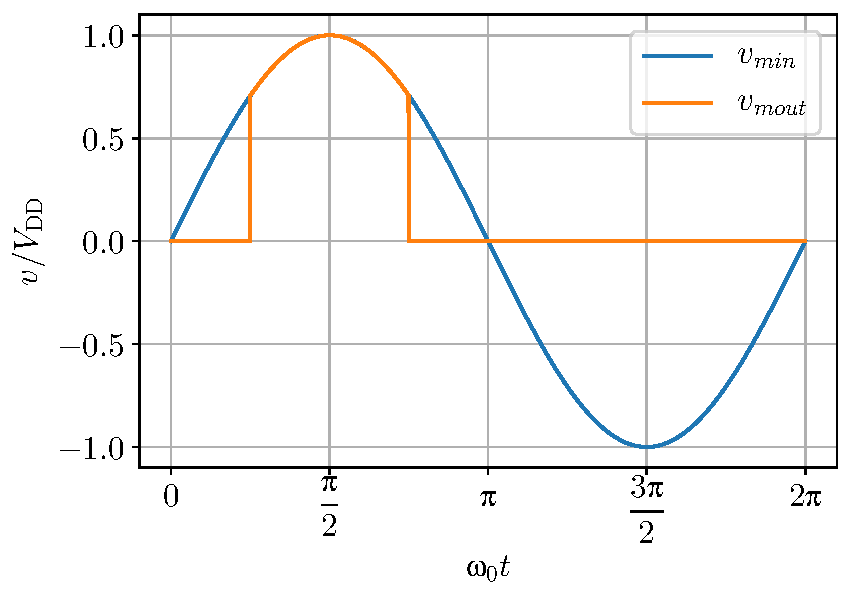
\includegraphics[scale=0.4]{fig/T2_a.pdf}
    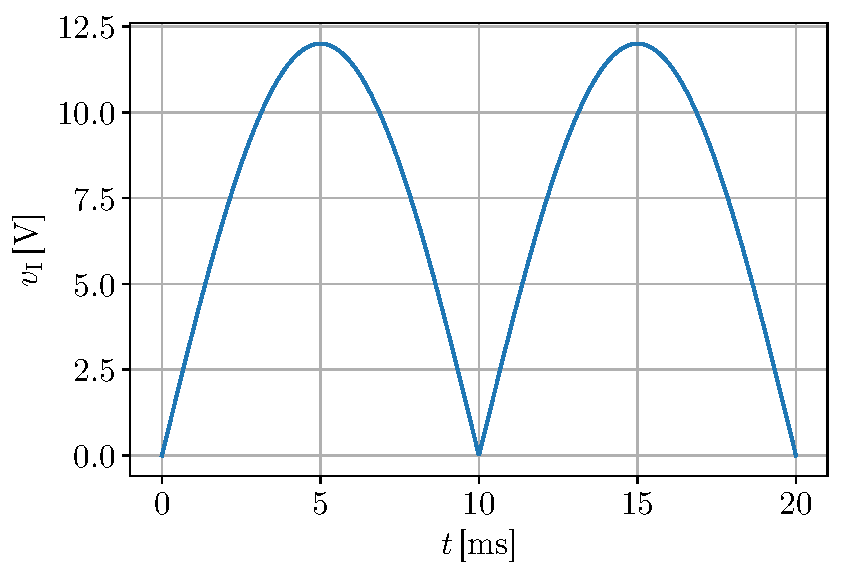
\includegraphics[scale=0.4]{fig/T2_b.pdf} \\
    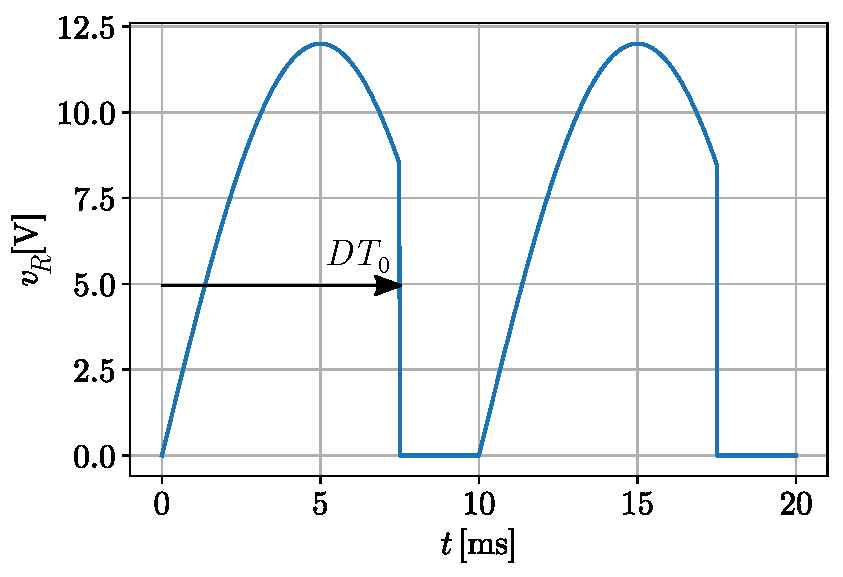
\includegraphics[scale=0.4]{fig/T2_c.pdf} \\
\end{center}
(б) $V_{\rm I}[k] = 
\dfrac{
\bigl(
\cos(\uppi D) + 
{\rm j}2k \sin(\uppi D) 
\bigr)
{\rm e}^{-{\rm j}2\uppi kD }
-1 }{\uppi(4k^2 - 1)}$